%\documentclass[]{article}
%\usepackage{natbib}
\documentclass[extra,mreferee]{gji}
%\documentclass[extra]{gji}
\usepackage{timet}
\usepackage{amsmath}
\usepackage{graphicx}
\usepackage{url}
\usepackage[utf8]{inputenc}

\usepackage{todonotes}

% Document metadata
% =================
\newcommand{\Title}{
    Non-linear gravity inversion in spherical coordinates:
    application to the South American Moho
}
\newcommand{\Keywords}{
        Moho;
        gravity inversion;
        spherical coordinates;
        tesseroid;
        South America
}
\title[]{\Title}
\author[]{
    Leonardo Uieda$^{1,2}$,
    Valéria C. F. Barbosa$^{2}$
    \\
    $^1$Universidade do Estado do Rio de Janeiro, Rio de Janeiro, Brazil.
    e-mail: leo@leouieda.com
    \\
    $^2$Observatório Nacional, Rio de Janeiro, Brazil.
}

\usepackage[pdftex,colorlinks=true]{hyperref}
\hypersetup{
    pdftitle={\Title},
    pdfauthor={Leonardo Uieda (leo@leouieda.com)},
    pdfsubject={},
    pdfkeywords={\Keywords},
    pdfcreator={pdfTeX},
    allcolors=blue,
}


% Useful commands
% ===============


\begin{document}

%\label{firstpage}
\maketitle


\begin{abstract}
\end{abstract}

\noindent\textbf{Key words:} \Keywords


%%%%%%%%%%%%%%%%%%%%%%%%%%%%%%%%%%%%%%%%%%%%%%%%%%%%%%%%%%%%%%%%%%%%%%%%%%%%%%%
\section{Introduction}


%%%%%%%%%%%%%%%%%%%%%%%%%%%%%%%%%%%%%%%%%%%%%%%%%%%%%%%%%%%%%%%%%%%%%%%%%%%%%%%
\section{Methodology}

In potential field methods,
we must isolate the target anomalous density distribution prior to modeling and
inversion.
In our case, the target is the relief of the real Moho undulating around a
reference Moho.
We do this by removing all other effects from the gravity observations.
The first correction is to remove the
gravity\footnote{The term ``gravity'' refers the sum of the gravitational and
centripetal accelerations.}
of an ellipsoidal Earth (the Normal Earth or reference ellipsoid).
This is done using the closed-form solution presented in
\citet{li_ellipsoid_2001}.
\todo{Needs review}
The resulting quantity is known as the gravity disturbance,

\begin{equation}
    \delta(P) = g(P) - \gamma(P)
\end{equation}

\noindent in which $g(P)$ is the measured gravity at an observation point $P$
and $\gamma(P)$ is the gravity of the Normal Earth
calculated at point $P$.

We assume that the crust of our Normal Earth has a standard density of
$\rho_{crust} = 2670\ kg.m^{-3}$ and a depth to the Moho of $z_{ref}$.
The disturbance contains only the gravitational effects of density
distributions that are anomalous with respect to the Normal Earth.
This includes all masses above the surface of the ellipsoid (the topography),
the mass deficiency of the oceans,
the mass deficiency of sedimentary basins,
crustal sources (e.g., igneous intrusions, lateral density changes, etc),
heterogeneities below the upper mantle,
and
the effect of the difference between the real Moho
topography and the reference Moho ($z_{ref}$).
In order to invert for the Moho topography, all effects must either be removed
or assumed negligible.

\subsection{Parametrization}

\begin{figure}
    \centering
    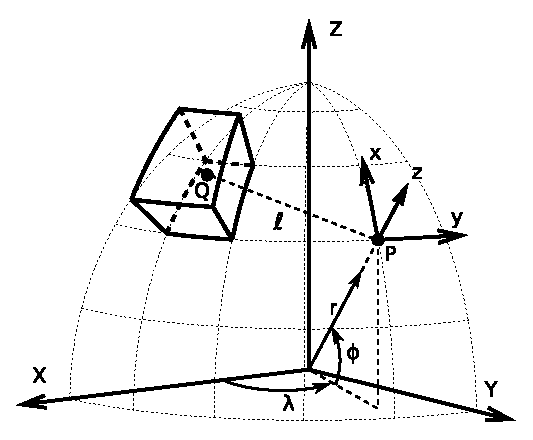
\includegraphics[width=\columnwidth]{figures/paper/tesseroid-coord-sys}
    \caption{Sketch of a tesseroid (spherical prism) in a geocentric coordinate
        system (X, Y, Z).
        Observations are made at point P with respect to it's local
        North-oriented coordinate system (x, y, z).
        After \citet{uieda_tesserioid_2015},
        available at
        \url{http://dx.doi.org/10.6084/m9.figshare.1495525}.
    }
    \label{fig:tess}
\end{figure}

We parameterize the forward problem by discretizing the Moho undulation
into a grid of $M_{lon} \times M_{lat} = M$ juxtaposed tesseroids (Fig.~\ref{fig:tess}).
\todo{Cite source separation figure}
In cases where the Moho is above the reference depth ($z_{ref}$),
the top of the tesseroid is the Moho depth at the location of the $k$-eth
tesseroid ($z_{k}$),
the bottom is $z_{ref}$, and the density-contrast is positive.
If the Moho is below the $z_{ref}$, the top of the tesseroid is $z_{ref}$,
the bottom is the Moho depth, and the density-contrast is negative.

Considering that the density-contrast of each tesseroid is fixed,
the predicted gravity anomaly of the Moho is a non-linear function of the
parameters $z_k$, $k=1, \ldots, M$,

\begin{equation}
    d_i = f_i(\mathbf{p}),
\end{equation}

\noindent in which $d_i$ is the $i$th element of the $N$-dimensional predicted
data vector $\mathbf{d}$, $\mathbf{p}$ is the $M$-dimensional parameter vector
containing the Moho depths ($z_k$),
and $f_i$ is the $i$th non-linear function that maps the parameters onto the
data.
$f_i$ is the radial component of the gravitational attraction of the tesseroid
model.
The gravitational attraction of a tesseroid is calculated using the
Gauss-Legendre Quadrature (GLQ) integration.
The accuracy of the GLQ integration is improved by an adaptive discretization
scheme.
\todo{Cite tesseroids paper.}


\subsection{Inverse problem}

We wish to estimate the parameter vector $\mathbf{p}$ from a set of observed
gravity anomaly data $\mathbf{d}^o$.
The least-squares estimate is the one that minimizes the data-misfit function

\begin{equation}
    \phi(\mathbf{p}) =
    [\mathbf{d}^o - \mathbf{d}(\mathbf{p})]^T[\mathbf{d}^o - \mathbf{d}(\mathbf{p})].
    \label{eq:data-misfit}
\end{equation}

Function $\phi(\mathbf{p})$ is non-linear with respect to $\mathbf{p}$.
Thus, we can find its minimum using gradient-based
iterative optimization
methods like the Gauss-Newton or Steepest Descent methods.
Such methods start from an initial estimate $\mathbf{p}^0$ and repeatedly update
the estimate until a minimum is reached.

For the Gauss-Newton method,
the update at the $k$th iteration $\mathbf{\Delta p} = \mathbf{p}^{k+1} - \mathbf{p}^k$
is the solution of the linear system

\begin{equation}
    \mathbf{H}^k\mathbf{\Delta p} = -\mathbf{g}^k,
    \label{eq:gaussnewton}
\end{equation}

\noindent in which
$\mathbf{g}^k$ and $\mathbf{H}^k$ are, respectively,
the gradient vector and the Hessian matrix of $\phi(\mathbf{p})$.

The Steepest Descent method uses only the gradient direction
to update the initial estimate

\begin{equation}
    \mathbf{\Delta p} = -\mathbf{g}^k.
    \label{eq:steepest}
\end{equation}

\noindent
Thus, it does not require the computation and storage of the Hessian matrix
nor the solution of linear systems.
However, the Steepest Descent method has poor convergence when the
current solution is close to the minimum of the goal function
\citep{kelley_iterative_1987}.

The gradient vector and the Gauss-Newton approximation of the Hessian matrix
of $\phi(\mathbf{p})$ are, respectively,

\begin{equation}
    \mathbf{g}^k = -2\mathbf{A}^T[\mathbf{d}^o - \mathbf{d}(\mathbf{p}^k)],
    \label{eq:gradient}
\end{equation}

\noindent
and

\begin{equation}
    \mathbf{H}^k = 2\mathbf{A}^T\mathbf{A},
    \label{eq:hessian}
\end{equation}

\noindent in which
$\mathbf{A}$ is the Jacobian or sensitivity matrix,

\begin{equation}
    A_{ij} = \dfrac{\partial f_i}{\partial p_j}(\mathbf{p^k}).
    \label{eq:jacobian}
\end{equation}



\subsection{Regularization}

Non-linear inversions for the relief of an interface (like
the Moho) are ill-posed and required additional constraints in the form of
regularization \citep{silva_potential-field_2001}.
A common approach is to use the first-order Tikhonov regularization to impose
smoothness on the solution,

\begin{equation}
    \theta(\mathbf{p}) = \mathbf{p}^T\mathbf{R}^T\mathbf{R}\mathbf{p},
\end{equation}

\noindent where $\mathbf{R}$ is an $L \times M$ finite-difference matrix
representing the $L$ first-order differences between adjacent tesseroids.

The solution $\hat{\mathbf{p}}$ to the regularized inverse problem is the one that
minimizes the goal function

\begin{equation}
    \Gamma(\mathbf{p}) = \phi(\mathbf{p}) + \mu\theta(\mathbf{p}).
\end{equation}

\noindent
The regularization parameter $\mu$ controls the balance between fitting the
observed data and obeying the smoothness constraint.

The goal function $\Gamma(\mathbf{p})$ is also non-linear with respect to
$\mathbf{p}$ and can be minimized using the Gauss-Newton or Steepest Descent
methods.
The gradient vector and Hessian matrix of the goal function are, respectively,

\begin{equation}
    \mathbf{g}^k =
        -2\mathbf{A}^T[\mathbf{d}^o - \mathbf{d}(\mathbf{p}^k)] +
        2\mu\mathbf{R}^T\mathbf{R}\mathbf{p}^k,
    \label{eq:gradient-regul}
\end{equation}

\noindent and

\begin{equation}
    \mathbf{H}^k = 2\mathbf{A}^T\mathbf{A} + 2\mu\mathbf{R}^T\mathbf{R}.
    \label{eq:hessian-regul}
\end{equation}



\subsection{Bott's method}

\citet{bott_use_1960} developed an efficient method to determined the basement
relief of a sedimentary basin from gravity observations.
The method requires data on a regular grid of $N_x \times N_y = N$
observations.
The basement relief is then discretized into an equal grid of $M_x \times
M_y = M$ elements with $M_x = N_x$ and $M_y = N_y$.
Bott's iterative method starts with an initial estimate of the basement relief
$\mathbf{p}^0$ equal to the null vector and updates the estimate using the formula

\begin{equation}
    \mathbf{\Delta p} = \dfrac{\mathbf{d}^o - \mathbf{d}(\mathbf{p}^k)}{2\pi G \Delta \rho},
    \label{eq:bott}
\end{equation}

\noindent
in which $G$ is the gravitational constant and $\Delta \rho$ is the basin
density contrast.
The iterative process stops when the inversion residuals
$\mathbf{r} = \mathbf{d}^o - \mathbf{d}(\mathbf{p}^k)$ fall below the assumed noise level
of the data.

\citet{silva_fast_2014} showed that Bott's method can be formulated as
a special case of the Gauss-Newton method (Eq.~\ref{eq:gaussnewton})
by setting the Jacobian matrix (Eq.~\ref{eq:jacobian}) to

\begin{equation}
    \mathbf{A} = 2\pi G \Delta \rho \mathbf{I},
    \label{eq:bott-jacobian}
\end{equation}

\noindent
in which $\mathbf{I}$ is the identity matrix.
In this framework,
Bott's method uses a Bouguer plate approximation of the relief to
linearize the Jacobian matrix.
However, the non-linearity of the predicted data $\mathbf{d}(\mathbf{p}^k)$ is
preserved.

We propose that Bott's method can also be formulated as a special case of the
Steepest Descent method (Eq.~\ref{eq:steepest}) by setting the Jacobian matrix to

\begin{equation}
    \mathbf{A} = \dfrac{1}{4 \pi G \Delta \rho}\mathbf{I}.
    \label{eq:bott-steepest}
\end{equation}

One of the advantages of Bott's method over the traditional Gauss-Newton or
Steepest Descent is eliminating the computation and storage of the dense
Jacobian matrix $\mathbf{A}$.
In practice, the derivatives in Eq.~\ref{eq:jacobian} are often calculated through a
first-order finite-difference approximation.
Thus, evaluating $\mathbf{A}$ requires $2\times M \times N$ forward modeling
operations for each iteration of the gradient descent algorithm.
Bott's method also does not require the solution of equation systems.

A disadvantage of Bott's method is that it suffers from instability
\citep{silva_fast_2014}.
A common approach to solve this issue is to apply a smoothing filter, like a
moving average, to the unstable estimate.


\subsection{Regularized Bott's method in spherical coordinates}

Approximate the Jacobian by making tesseroid size tend to infinity to get
Bouguer slab.
This approximation is good for tesseroids because each will cover a large
enough area.
Show case for the Steepest Descent.
Extend the Jacobian to include lateral density variation.
Important because density-contrast is positive or negative depending if the
Moho is above or below the reference level.
Enforce that the use of a particular

Biggest computation time is in forward modeling.
All matrices involved are sparse.
Solve the sparse linear system with a conjugate gradient method.
\todo{Check which conjugate gradient scipy.space.linalg.solve uses.}
Use the regularized inversion because multiplying and solving the linear system
are fast compared to forward modeling.
Not using step size optimization because forward modeling is very slow so
increased convergence doesn't justify the extra time spent on the discarded
step attempts.

\subsection{Determination of hyper-parameters}



\subsection{Software implementation}

\todo{Cite packages in the references.txt file.}


%%%%%%%%%%%%%%%%%%%%%%%%%%%%%%%%%%%%%%%%%%%%%%%%%%%%%%%%%%%%%%%%%%%%%%%%%%%%%%%
\section{Application to synthetic data from a simple model}


Meh.


%%%%%%%%%%%%%%%%%%%%%%%%%%%%%%%%%%%%%%%%%%%%%%%%%%%%%%%%%%%%%%%%%%%%%%%%%%%%%%%
\section{Application to synthetic data from the CRUST1.0 model}

Meh.


%%%%%%%%%%%%%%%%%%%%%%%%%%%%%%%%%%%%%%%%%%%%%%%%%%%%%%%%%%%%%%%%%%%%%%%%%%%%%%%
\section{Application to the South American Moho}


\subsection{Gravity data}

The gravitational effect of the topography
is removed using the
ETOPO1\footnote{\url{http://dx.doi.org/10.7289/V5C8276M}}
digital terrain model
\citep{amante_c._and_b._w._eakins_etopo1_2009}.
The effect of sedimentary basins is removed using the
CRUST1.0\footnote{\url{http://igppweb.ucsd.edu/~gabi/rem.html}} model
by
\citet{laske_update_2013}.
Lateral variations in density along the Moho cannot be properly accounted for
in regions where information coverage is sparse and readily accessible models
are not available, like in the South American and African continents.
For the purposes of this study, we will assume that all other crustal sources
and lateral variations in density are negligible.


\begin{figure*}
    \centering
    \includegraphics[width=\textwidth]{figures/paper/sam-gravity-data}
    \caption{This is a figure caption.}
    \label{fig:sam-data}
\end{figure*}

\begin{figure*}
    \centering
    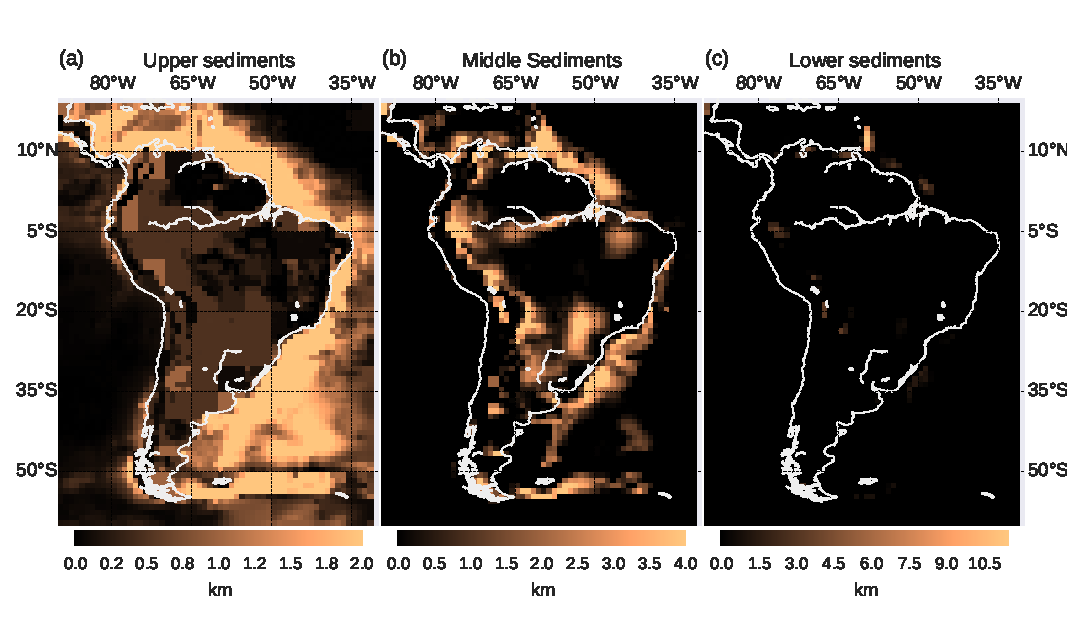
\includegraphics[width=\textwidth]{figures/paper/sam-gravity-sed}
    \caption{This is a figure caption.}
    \label{fig:sam-sed}
\end{figure*}


\subsection{Inversion results}

%%%%%%%%%%%%%%%%%%%%%%%%%%%%%%%%%%%%%%%%%%%%%%%%%%%%%%%%%%%%%%%%%%%%%%%%%%%%%%%
\section{Discussion}

Meh.

%%%%%%%%%%%%%%%%%%%%%%%%%%%%%%%%%%%%%%%%%%%%%%%%%%%%%%%%%%%%%%%%%%%%%%%%%%%%%%%
\section{Conclusions}

Meh.

%%%%%%%%%%%%%%%%%%%%%%%%%%%%%%%%%%%%%%%%%%%%%%%%%%%%%%%%%%%%%%%%%%%%%%%%%%%%%%%
\section{Acknowledgments}

Meh.

\bibliographystyle{gji}
\bibliography{biblio}

\end{document}
